\chapter{Figuras e Tabelas}
\label{ch:Misch}

O \LaTeX permite gerir a lista de figuras e tabelas de forma automática. O primeio passo consiste em criar as
 devidas imagems e tabelas, associando a cada uma delas um identificador único.

Por exemplo, a Tabela \ref{tab:umaTabela} apresenta os dados obtidos na experiência \ldots
\begin{table}[h]
	\centering
	\caption{Uma tabela}
	\begin{tabular}{ c c c c }
		\hline \hline
		$c_1$ & $c_2$ & $c_3$ & $\sum_{i=1} c_i$ \\
		\hline \hline
		$1$ & $2$ & $3$ & $6$ \\
		$1.1$ & $2.2$ & $3.3$ & $6.6$ \\
		\hline \hline
	\end{tabular}
	\label{tab:umaTabela}
\end{table}

A Tabela \ref{tab:umaTabela} é outro exemplo de uma tabela com barras verticais a separar as várias colunas.

\begin{table}[h]
	\centering
	\caption{Outra tabela com barras verticais}
	\begin{tabular}{ c|c|c|c }
		\hline \hline
		$c_1$ & $c_2$ & $c_3$ & $\sum_{i=1} c_i$ \\
		\hline \hline
		$1$ & $2$ & $3$ & $6$ \\
		$1.1$ & $2.2$ & $3.3$ & $6.6$ \\
		\hline \hline
	\end{tabular}
	\label{tab:outraTabela}
\end{table}

Para além de tabelas também é possivel apresentar figuras. Por exemplo, a Figura \ref{fig:umafigura} descreve \ldots
\begin{figure}[h]
	\centering
	
\includegraphics[width=2cm]{./fig_logo_ISEL}
	\caption[Uma figura com duas legendas]{Uma figura com duas legendas. A versão curta apenas aparece no índice de figuras}
	\label{fig:umafigura}
\end{figure}

\paragraph{Atenção.} Todas as tabelas e figuras, e.g., diagramas, imagens ilustrativas da aplicação em funcionamento, têm que ser devidamente enquadradas no texto antes de serem apresentadas e esse enquadramento inclui uma explicação da imagem apresentada e eventuais conclusões (interpretações) a tirar dessa imagem.

\mbox{} \\

A Figura \ref{fig:umafiguraR} apresenta um exemplo de uma figura que é apresentada numa página rodada 90º.

\begin{landscape}
\begin{figure}[h!]
	\centering
	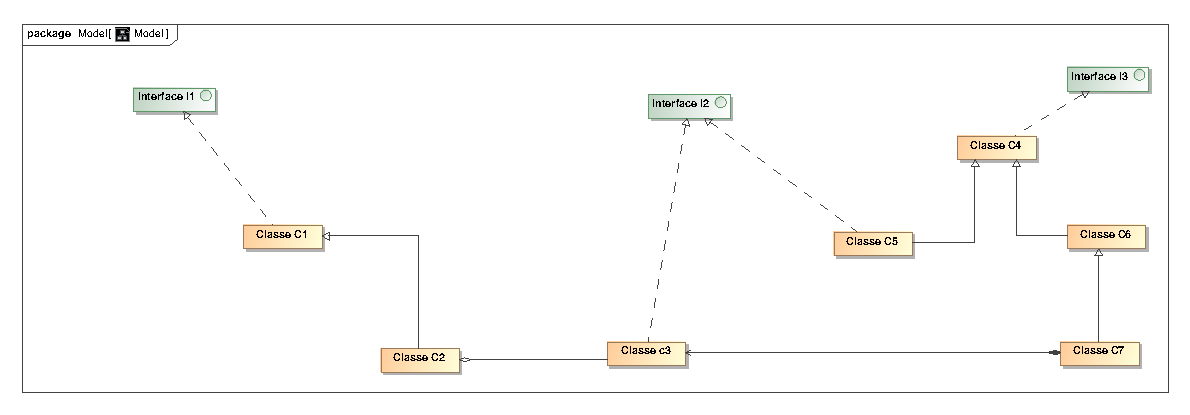
\includegraphics{./Model.eps}
	\caption{Figura rodada}
	\label{fig:umafiguraR}
\end{figure}
\end{landscape}

E mais texto depois da figura.